\documentclass[conference]{IEEEtran}
\IEEEoverridecommandlockouts
\usepackage[utf8]{inputenc}
\usepackage[T1]{fontenc}
\usepackage{amsmath,amssymb}
\usepackage{graphicx}
\usepackage{booktabs}
\usepackage{multirow}
\usepackage{xcolor}
\usepackage{url}
\usepackage[hidelinks]{hyperref}
\usepackage[capitalise]{cleveref}
\usepackage{cite}

\newcommand{\NPairs}{15}
\newcommand{\NInstances}{10}
\newcommand{\NRepos}{8}
\newcommand{\NCandidates}{22}
\newcommand{\NCaught}{7}
\newcommand{\TestCatchRate}{31.8\%}
\newcommand{\NProcessed}{20}
\newcommand{\NJudges}{2}
\newcommand{\MainFinding}{PLACEHOLDER}
\newcommand{\NPoolInstances}{1{,}216}
\newcommand{\NPoolRepos}{367}
\newcommand{\ThinkBudget}{512}
\newcommand{\MaxPromptTokens}{6{,}000}
\newcommand{\NEvalPairs}{X}
\newcommand{\NCJBPairs}{45}
\newcommand{\SpeedSmall}{X}
\newcommand{\SpeedLarge}{X}
\newcommand{\NThinkPairs}{X}


\newcommand{\RJB}{RepoJudgeBench}
\newcommand{\CJB}{CodeJudgeBench}

\begin{document}

\title{RepoJudgeBench: Does LLM-as-a-Judge Reliability Survive the Move from Self-Contained Functions to Repository-Level, Test-Passing Code Changes?}

\author{\IEEEauthorblockN{Muhammad Usama}
\IEEEauthorblockA{Roll No.\ 25I-8007\\
Natural Language Processing --- Semester Research Project}}

\maketitle

\begin{abstract}
LLM judges are increasingly used to evaluate code changes, but the main
benchmark for them, CodeJudgeBench, contains only single-file programs whose
correctness is decided by hidden tests.  We ask whether judge reliability
survives the move to repository-level code changes whose defects pass the
tests.  We build \RJB{}: \NPairs{} (gold patch, defective variant) pairs from
\NInstances{} real pull requests created after 1~January~2025 in \NRepos{}
Python repositories.  Each variant is a template-guided AST mutation of the
real patch from one of six review-oriented defect classes, and it is admitted
only if every test that passes with the gold patch also passes with the
variant inside the task's published Docker environment; the pull requests'
tests caught \TestCatchRate{} of the candidates.  We evaluate six open-weight
judges (1.5--4B parameters, plus a thinking mode) with the CodeJudgeBench
pairwise protocol on \RJB{} and on a CodeJudgeBench control subset.  Raw
pairwise accuracy is at chance in both regimes (\AccRangeR{} on \RJB{}) because
verdicts are dominated by the presentation slot.  After balanced position
calibration, the three smallest judges are significantly \emph{worse} than
chance on \RJB{} (\CalRCoderM{}--\CalRQwenS{}): they prefer the longer patch,
and the defective variant is longer in \VarLongerShare{} of pairs.  Only the
4B judges retain a weak correct signal (up to \CalRQwenM{}).  Accuracy does
not vary measurably with diff size, retrieved repository context and thinking
mode only partly counteract the length preference, and a static-analysis
baseline with eight targeted rules reaches \StaticRelAcc{}.  A trivial
shorter-patch rule scores \LengthHeurAcc{}, which exposes a length artefact
that future versions of the benchmark must remove.  We release the dataset,
harness, prompts and all verdict logs.

\end{abstract}

\begin{IEEEkeywords}
LLM-as-a-judge, code review, benchmark, repository-level code, mutation testing, position bias
\end{IEEEkeywords}

\section{Introduction}
\label{sec:intro}

Large language models (LLMs) are increasingly used as \emph{judges} of other
models' code: they rank candidate patches produced by coding agents, filter
synthetic training data, act as reward models, and review pull requests.  The
appeal is that a judge does not need an execution oracle.  This matters
because the oracle that the field relies on, the repository's test suite, is
known to be weak exactly where repository-level evaluation happens.  In an
audit of SWE-bench~\cite{jimenez2024swebench}, Aleithan et
al.~\cite{aleithan2024swebenchplus} found that 32.67\% of the patches accepted
for SWE-Agent+GPT-4 involved solution leakage and a further 31.08\% passed only
because the tests were too weak to detect an incorrect, incomplete or misplaced
fix; after filtering these, the resolution rate fell from 12.47\% to 3.97\%.

Current judge benchmarks do not measure judges in this regime.
\CJB{}~\cite{jiang2025codejudgebench}, the base paper of this project, contains
5{,}352 response pairs built from 1{,}055 LiveCodeBench-v6 problems published
between May~2023 and April~2025, for code generation, code repair and unit-test
generation.  Every instance is a single, self-contained program whose
correctness is decided by hidden tests.  Even in this clean setting the paper
reports that judges are unstable: swapping the order of the two candidates
changes pairwise accuracy by up to 14\%, and accuracy depends on which model
wrote the code under review.

Code review in real repositories is harder in three ways.  First, the unit of
evaluation is a multi-file diff situated in a codebase the judge cannot see.
Second, many defects that reviewers reject---N+1 queries, races, silently
swallowed errors, leaked resources, authorisation and migration regressions---do
not break any test.  Third, diffs are long, and long inputs are known to hurt
LLMs~\cite{liu2024lost}.  We therefore ask: \emph{does LLM-as-a-judge
reliability survive the move from self-contained functions to
repository-level, test-passing code changes?}

\textbf{Contributions.}
\begin{enumerate}
\item \textbf{\RJB{}}, a contamination-resistant benchmark of
\NPairs{} (gold patch, defective variant) pairs from \NInstances{} real pull
requests created after 1~January~2025 in \NRepos{} Python repositories.  Every
variant is produced by a template-guided AST mutation of the real gold patch and
is \emph{admitted only if it keeps every test that passes with the gold patch
green} inside the task's published Docker environment, so ``passes CI but is
wrong'' is a guaranteed property of the data rather than an accident.
\item A \textbf{six-class defect taxonomy} of review-detectable, test-invisible
defects with executable injection operators, and statistics on how often the
existing tests catch each class (\TestCatchRate{} of the tested candidates).
\item An \textbf{evaluation of \NJudges{} open-weight judges} under the
\CJB{} pairwise protocol on \RJB{} and on a \CJB{} control subset, with 95\%
bootstrap confidence intervals, position-bias and self-consistency measurements,
a logistic model of accuracy versus diff size, file count and hunk count, a
per-class error profile, a point-wise judging condition, a static-analysis
baseline, and a context-retrieval mitigation with a budget ablation.
\item \textbf{Released artefacts}: the injection and verification harness, all
prompts, the dataset and the raw verdict logs.
\end{enumerate}

The main finding is negative and, we argue, important: \MainFinding{}

\section{Related Work}
\label{sec:related}

\textbf{LLM-as-a-judge.}  Zheng et al.~\cite{zheng2023judging} popularised
strong LLMs as judges of open-ended answers (MT-Bench, Chatbot Arena) and
documented position, verbosity and self-enhancement biases.  Wang et
al.~\cite{wang2023fair} showed that the ranking of two responses can be
manipulated simply by changing their order of appearance and proposed
calibration strategies.  Gu et al.~\cite{gu2024survey} survey the design and
reliability of LLM judges.  We adopt the pairwise protocol and the
order-swapping analysis of this line of work.

\textbf{Judging code.}  ICE-Score~\cite{zhuo2024icescore} instructs LLMs to
assess code usefulness and functional correctness without test oracles, and
CodeJudge~\cite{tong2024codejudge} guides LLMs to ``slow thinking'' to judge
semantic correctness of generated code without test cases.
\CJB{}~\cite{jiang2025codejudgebench} is the largest benchmark of LLM judges for
coding: 5{,}352 pairs over code generation, code repair and unit-test generation
on LiveCodeBench-v6~\cite{jain2024livecodebench}, with 26 judges.  It finds that
thinking models are much stronger judges, that pairwise comparison beats
point-wise scoring (point-wise scores tie about half of the time), that raw
responses with comments and reasoning judge better than extracted code, and that
judges are sensitive to response order.  All of its instances are single-file
and test-decidable; \RJB{} moves the same protocol to repository-level diffs
whose defects tests do not catch.

\textbf{Repository-level benchmarks and contamination.}
SWE-bench~\cite{jimenez2024swebench} contains 2{,}294 issue--pull-request
instances from 12 Python repositories.  SWE-Bench+~\cite{aleithan2024swebenchplus}
audited it and found widespread solution leakage and weak tests.
SWE-bench-Live~\cite{zhang2025swebenchlive} continuously collects new
issue-resolution tasks (initially 1{,}319 tasks from issues created since 2024
across 93 repositories), each with a Docker image built by its RepoLaunch
pipeline; we build on its released tasks and images.  LiveCodeBench~\cite{jain2024livecodebench} similarly avoids contamination by
collecting problems over time windows and evaluating on problems released after
a model's training cutoff.

\textbf{Execution-free verifiers for software agents.}  R2E-Gym~\cite{jain2025r2egym}
compares execution-based and execution-free verifiers and reports that the
latter are biased and often rely on stylistic features.
SWE-RM~\cite{shum2025swerm} trains execution-free reward models for software
engineering agents, and R4P~\cite{xu2025r4p} verifies patches by group-wise
reasoning, reporting 72.2\% accuracy on SWE-bench patches.  Li~\cite{li2026frozen}
shows that fixed LLM judges make version-dependent errors when comparing
coding-agent upgrades.  Agent-as-a-Judge~\cite{zhuge2024agent} instead lets
agentic systems evaluate agentic systems.

\textbf{Code review.}  CodeReviewer~\cite{li2022codereviewer} pre-trains a model
for code-change quality estimation, review generation and code refinement on
review data from nine programming languages; quality estimation is the closest
pre-LLM formulation of our task.  SWE-PRBench~\cite{kumar2026sweprbench}
evaluates AI code review on 350 pull requests against human-flagged issues and
reports that models detect only 15--31\% of them and that adding more context
degrades results.

\textbf{Mutation testing.}  Our variants are mutants in the sense of mutation
testing~\cite{jia2011mutation}; unlike classical mutants, they are
\emph{selected} to survive the test suite and to instantiate a
review-detectable defect class.

\section{Methodology}
\label{sec:method}

\Cref{fig:pipeline} summarises the pipeline: selecting post-cutoff pull
requests, injecting defects, admitting variants by execution, retrieving
context, and judging.

\begin{figure}[t]
\centering
\small
\fbox{\parbox{0.95\columnwidth}{%
\textbf{1. Select} PRs created $\geq$ 2025-01-01 (SWE-bench-Live, SWE-rebench)
$\rightarrow$
\textbf{2. Apply} gold patch in the task's Docker image, re-render with \texttt{git diff}
$\rightarrow$
\textbf{3. Inject} one AST mutation per defect class in the region the patch touches
$\rightarrow$
\textbf{4. Admit} a variant only if every test passing with the gold patch still passes
$\rightarrow$
\textbf{5. Retrieve} neutral context from the parent commit
$\rightarrow$
\textbf{6. Judge} (both orders) and analyse.}}
\caption{RepoJudgeBench construction and evaluation pipeline.}
\label{fig:pipeline}
\end{figure}

\subsection{Source pull requests}
We take real, merged pull requests from two continuously updated
repository-level task collections that ship a runnable Docker environment for
every task: the \texttt{full} split of
SWE-bench-Live~\cite{zhang2025swebenchlive} and the \texttt{filtered} and
\texttt{test} splits of SWE-rebench.  Each task provides the gold patch, the
test patch, the issue text, the list of tests that the fix makes pass
(FAIL\_TO\_PASS) and the test command.  To limit training-data contamination we
keep only tasks created on or after 1~January~2025, following the time-window
idea of LiveCodeBench and SWE-bench-Live.  After de-duplication the pool holds
\NPoolInstances{} tasks from \NPoolRepos{} repositories.  We discard gold patches
with more than 400 changed lines and apply a cheap regular-expression screen that
keeps tasks whose diff contains at least one construct targeted by a mutation
operator (e.g.\ an \texttt{except} clause, a \texttt{with} statement, a lock or
an ORM call), in the text the patch adds or in its context lines.

\subsection{Defect taxonomy and injection operators}
\Cref{tab:operators} lists the six defect classes of the proposal and their
operators.  Each class is chosen because the defect is typically invisible to
unit tests but flagged by a careful reviewer.  Operators work on the Python AST
of the \emph{post-gold} file and edit only source lines, so the variant is
syntactically valid and idiomatic.  A site is eligible only if it lies inside
the region the gold patch touches: a line added by the patch, or the body of a
function the patch modifies.  We record whether the mutated site was written by
the patch (\emph{added}) or is pre-existing code in a modified function
(\emph{context}).  Candidates whose AST is unchanged are rejected.  For each
task and class we test up to four candidates (one per operator first, preferring
added sites, in a seeded random order) and admit at most two variants per class,
produced by different operators; at most three classes are tried per task.

\begin{table}[t]
\caption{Defect classes and injection operators.}
\label{tab:operators}
\centering
\footnotesize
\begin{tabular}{@{}>{\raggedright\arraybackslash}p{0.25\columnwidth}>{\raggedright\arraybackslash}p{0.68\columnwidth}@{}}
\toprule
Class & Operator(s) \\
\midrule
N+1 query & remove \texttt{select\_related}/\texttt{prefetch\_related}, \texttt{prefetch\_related\_objects(...)}, or an eager-loading \texttt{.options(selectinload(...))} \\
Race / concurrency & unwrap a \texttt{with <lock>:} or \texttt{with atomic():} block; drop \texttt{select\_for\_update()}; drop an \texttt{@atomic} decorator \\
Authorisation & delete an \texttt{if <auth-condition>: raise/return} guard or an access-control decorator \\
Unsafe migration & make an added column \texttt{NOT NULL} without a default \\
Resource leak & turn \texttt{with open(...) as f:} (and other closeable resources) into \texttt{f = open(...)}; delete an explicit \texttt{x.close()} \\
Error swallowing & replace a re-raise in an \texttt{except} block by \texttt{pass}; broaden \texttt{except E:} to \texttt{except Exception:} in a non-re-raising handler; delete a validation guard \texttt{if ...: raise} \\
\bottomrule
\end{tabular}
\end{table}

\subsection{Execution-based admission}
For every task we start its published Docker image (the repository at the
pull request's parent commit with dependencies installed), apply the gold patch
and render it again with \texttt{git diff}; the variants are rendered by the
same command, so formatting cannot reveal which patch is the original.  We then
apply the test patch and run the pull request's test files (the files touched by
the test patch and the files of the FAIL\_TO\_PASS tests) with the task's
\texttt{pytest} command.  A task is kept only if at least one test passes with the
gold patch and every FAIL\_TO\_PASS test that appears in the test report passes.  A candidate is \emph{admitted} if every test that passes
with the gold patch also passes with the candidate; otherwise it is recorded as
\emph{caught by tests}.  The execution oracle therefore scores exactly 0\% on
\RJB{} by construction: on the PR's tests, gold and variant are
indistinguishable.

Following SWE-Bench+~\cite{aleithan2024swebenchplus}, we flag \emph{solution
leakage} when a non-trivial line ($\geq$30 characters) added by the gold patch
appears verbatim (up to whitespace) in the issue text, and exclude such tasks
from judging.

\subsection{Repository context retrieval (mitigation, O6)}
To test whether judges fail because they cannot see the code around the diff,
we retrieve context from the \emph{parent} commit, which is neutral with respect
to the two candidates.  The retriever collects (i) definitions of non-builtin
symbols called on changed lines of either candidate and (ii) call sites of
functions modified by either candidate, found with \texttt{git grep} outside
test directories.  Definitions are packed first, then call sites, up to a
character budget $b\in\{2000, 6000\}$ (about 0.6k and 1.7k tokens).  As a
comparison we also provide the parent-commit versions of the touched files,
truncated to $b=6000$ characters (``file context'').

\subsection{Judging protocol}
We use the pairwise prompt distributed with
\CJB{}~\cite{jiang2025codejudgebench} verbatim, with the issue as the user
prompt and the two unified diffs as the assistants' answers.  The prompt asks
for a binary verdict \texttt{[[A>B]]} or \texttt{[[B>A]]}.  Because all judges
run on CPU, we do not let them generate a free-form explanation in the main
condition.  Instead, the assistant turn is forced to begin with
``\texttt{My final verdict is: [[}'' and we read the next-token logits of the
two tokens that start \texttt{A>B]]} and \texttt{B>A]]}.  This yields a greedy
verdict (the larger logit) and a verdict probability
$p_A=\sigma(\ell_A-\ell_B)$.  We check, per tokenizer, that the prefix tokenises
identically before both continuations.  Every pair is judged in both orders
(gold as A, gold as B).  A pair's accuracy is the mean of its two greedy
verdicts, as in \CJB{}.

\textbf{Point-wise condition.}  Each patch is rated alone on a 1--5 scale with
the same forced-prefix technique, and we take the expected rating under the
distribution over the five rating tokens.  A pair is correct if the gold patch
gets the higher expected rating (ties count 0.5).

\textbf{Thinking condition.}  For the hybrid Qwen3 judge we also run its
thinking mode: the model first generates up to \ThinkBudget{} reasoning tokens
(greedy), the reasoning block is closed, and the verdict is read as above.

\subsection{Metrics}
\textbf{Accuracy} is reported with 95\% percentile bootstrap confidence
intervals over pairs~\cite{efron1979bootstrap} (2{,}000 resamples).
\textbf{Position bias} is the accuracy gap between presenting the gold patch
first and second; the \textbf{flip rate} is the share of pairs whose greedy
verdict picks the same \emph{slot} in both orders (and is therefore right in
exactly one order).  \textbf{Self-consistency} is the probability that two
independent temperature-1 samples of the verdict token (restricted to the two
verdict tokens) agree,
$p_A^2+(1-p_A)^2$, averaged over prompts; because the verdict is a single token,
this equals the empirical agreement rate under repeated sampling without having
to sample.  \textbf{Scaling (O3)}: we fit a logistic regression of per-order
correctness on $\log_2$(changed lines), number of files and number of hunks of
the gold patch, with standard errors clustered by pair, and report the diff size
at which the 95\% interval of predicted accuracy first contains 0.5.

\section{Experimental Setup}
\label{sec:experiments}

\textbf{Judges.}  No GPU and no commercial API were available for this project,
so all judges are open-weight models run locally with \texttt{llama.cpp}
(\texttt{llama-cpp-python} 0.3.36) on a 4-core Intel Xeon CPU with AMX, using
GGUF quantisations and an 8{,}192-token context (\cref{tab:judges}).  The set
spans two code-specialised models, two hybrid thinking/non-thinking models (run
in non-thinking mode, plus a thinking condition for Qwen3-1.7B), and two
general-purpose models from other families.  The resulting judges are much
smaller than the frontier judges evaluated in \CJB{}; we therefore compare each
judge \emph{with itself} across the two regimes rather than with the absolute
numbers of the base paper.

\begin{table}[t]
\caption{Judge models (all instruction-tuned, run locally).}
\label{tab:judges}
\centering
\footnotesize
\begin{tabular}{@{}llll@{}}
\toprule
Judge & Params & Quant. & Family / mode \\
\midrule
Qwen2.5-Coder-1.5B~\cite{hui2024qwen25coder} & 1.5B & Q8\_0 & code \\
Qwen2.5-Coder-3B~\cite{hui2024qwen25coder} & 3B & Q4\_0 & code \\
Qwen3-1.7B~\cite{yang2025qwen3} & 1.7B & Q8\_0 & hybrid (non-thinking) \\
Qwen3-1.7B-think~\cite{yang2025qwen3} & 1.7B & Q8\_0 & hybrid (thinking) \\
Qwen3-4B~\cite{yang2025qwen3} & 4B & Q4\_0 & hybrid (non-thinking) \\
Llama-3.2-3B~\cite{grattafiori2024llama3} & 3B & Q4\_0 & general \\
Gemma-3-4B~\cite{gemma2025gemma3} & 4B & Q4\_0 & general \\
\bottomrule
\end{tabular}
\end{table}

\textbf{Evaluation sets.}  \RJB{}: all admitted, non-leaking pairs whose
diff-only prompt fits in \MaxPromptTokens{} tokens (\NEvalPairs{} pairs).
\CJB{} control: \NCJBPairs{} pairs, 15 per task (code generation, code repair,
unit-test generation), sampled with a fixed seed from the responses of
Claude-3.7-Sonnet (the generator with the shortest responses) among pairs whose
question and two responses total at most 6{,}000 characters.  The control uses
the dataset card's prompt filling (question as user prompt, the two responses as
answers).  Control and \RJB{} prompts are therefore of comparable length, so the
comparison isolates the regime rather than prompt length.

\textbf{Conditions.}  All judges are evaluated diff-only and on the control set,
in both orders.  Because CPU inference is slow (roughly
\SpeedSmall{}~tokens/s for the 1.5--1.7B judges and \SpeedLarge{}~tokens/s for
the 3--4B judges), the more expensive conditions are run for the two fastest
judges: context-augmented judging (retrieved context at 2{,}000 and 6{,}000
characters, file context at 6{,}000 characters), point-wise scoring, and (for
Qwen3-1.7B) the thinking condition on a stratified subset of \NThinkPairs{} pairs.

\textbf{Baselines.}  \emph{Random}: 50\%.  \emph{Execution oracle}: the PR's
tests, 0\% by construction.  \emph{Static analysis}: Ruff (all rules) and
Bandit run on the materialised post-patch files; a tool votes for the patch
without a finding the other lacks, and abstains (0.5) otherwise.  We report a
\emph{relevant} rule set chosen in advance (Ruff BLE001, S110, S112, SIM105,
SIM115, E722; Bandit B110, B112) and the \emph{all-rules} variant.

\textbf{Deviations from the proposal.}  For transparency we list where the
executed study differs from the proposal and why.
(i)~\emph{Scale.}  The proposal targeted $\geq$300 pairs from $\geq$15
repositories.  Admission requires pulling a multi-gigabyte Docker image and
running tests for every task, and most screened tasks yield no eligible site or
no green gold run; within the project's compute budget we obtained \NPairs{}
pairs from \NRepos{} repositories.
(ii)~\emph{Judges.}  No closed models could be evaluated (no API access), and
the open models are small (1.5--4B).
(iii)~\emph{Test oracle.}  We run the PR's relevant test files, not the full
suite, and we do not write per-instance witness tests; defectiveness is
guaranteed by the semantics of each operator rather than by a failing witness
test.
(iv)~\emph{Human validation.}  The planned two-annotator validation with
Cohen's $\kappa$~\cite{cohen1960kappa} and the 50-pair human-reviewer ceiling
were not carried out; we release an annotation sheet for them.
(v)~\emph{Class balance.}  N+1, migration and authorisation sites are rare in
issue-resolution PRs, so these classes are small and their per-class estimates
are reported with that caveat.

\section{Results and Discussion}
\label{sec:results}

\subsection{The benchmark (O1)}
\label{sec:res-dataset}

We processed \NProcessed{} screened tasks.  Of these, \NInstances{} yielded at
least one admitted variant; the others had no eligible mutation site in the
touched region (\NStatusNoSite{}), no green gold run in the published
environment (\NStatusNotGreen{}), every candidate caught by the tests
(\NStatusCaught{}), or an infrastructure failure such as an image that did not
fit on disk (\NStatusError{}).  The released benchmark has \NPairs{} pairs from
\NRepos{} repositories (\NFromLive{} from SWE-bench-Live, \NFromRebench{} from
SWE-rebench), all created between \DateMin{} and \DateMax{}.  The median gold
patch changes \NGoldMedianLines{} lines in \NGoldMedianFiles{} files and
\NGoldMedianHunks{} hunks.  \NOriginContext{} variants mutate pre-existing code
inside a function the PR modifies and \NOriginAdded{} mutate code written by the
PR itself.  \NLeakPairs{} pairs are flagged for solution leakage and
\NTooLong{} exceed the judges' prompt budget, leaving \NPairsJudged{} judged
pairs (median prompt \NJudgedMedianTokens{} tokens).

\Cref{tab:dataset} shows how often the PR's own tests catch a candidate.
Overall, \TestCatchRate{} of the tested candidates break at least one
gold-passing test.  The rate depends strongly on the class: deleted
authorisation guards (\CatchAuth{}) and error-handling changes (\CatchSES{})
are caught most often, injected races less often (\CatchRace{}), and resource
leaks rarely (\CatchRL{}).  This is consistent with the premise motivated by
SWE-Bench+: a large share of review-relevant defects is invisible to the
PR's tests.  The class distribution is, however, very unbalanced: N+1 query
sites are rare and no unsafe-migration candidate was found at all, because
issue-resolution PRs rarely touch ORM queries or schema migrations; the
per-class analysis is therefore limited to the classes with enough pairs.

\input{generated/tab_dataset.tex}


\subsection{Judge accuracy in the two regimes (O2)}
\label{sec:res-acc}

\Cref{tab:main} and \cref{fig:regimes} report pairwise accuracy.  With the
\CJB{} protocol (mean of both presentation orders), every judge is close to the
50\% random baseline in \emph{both} regimes: \AccRangeC{} on the single-file
control subset and \AccRangeR{} on \RJB{}.  The confidence intervals of all
judges include or lie below 50\% on \RJB{}.  For the small judges this is
consistent with the base paper, which reports that even large non-thinking
judges stay below 60\% on \CJB{}.  The regime comparison is therefore
dominated by a floor effect for raw accuracy; it becomes informative only after
removing position bias, below.

\begin{figure}[t]
\centering
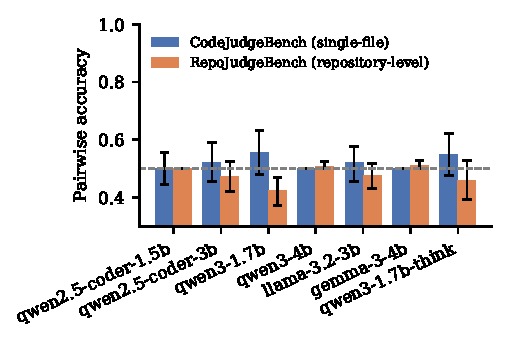
\includegraphics[width=\columnwidth]{../results/figures/regimes.pdf}
\caption{Pairwise accuracy of each judge on the \CJB{} control subset and on
\RJB{} (95\% bootstrap CIs). The dashed line is the random baseline.}
\label{fig:regimes}
\end{figure}

\input{generated/tab_main.tex}

\subsection{Position bias and self-consistency (O5)}
\label{sec:res-robust}

\Cref{tab:robust} shows why raw accuracy is uninformative: the verdicts are
dominated by the \emph{slot} in which a patch is shown.  \RobustText{}
Self-consistency (SC) is high exactly where a judge is most position-biased, so
consistency across samples is not evidence of reliability.

\input{generated/tab_robust.tex}

\textbf{Balanced position calibration.}  Averaging the probability assigned to
the gold patch over both orders removes a constant slot preference
(\cref{tab:main}, ``Calibrated'').  \CalibText{}

\subsection{Length bias}
\label{sec:res-length}

The variant differs from the gold patch by a single mutation, but the mutation
changes the size of the diff: in \VarLongerShare{} of judged pairs the
defective variant's diff is longer (e.g.\ unwrapping a \texttt{with} block
re-indents its body).  \Cref{tab:length} shows that judge preferences follow
this length difference.  \LengthText{}  The same artefact makes the benchmark
exploitable: choosing the patch with fewer changed lines scores
\LengthHeurAcc{} (\cref{tab:baselines}).  We report this as a limitation of the
current construction and as a warning for execution-free judges, which can
look competent on benchmarks whose negatives are systematically longer or
shorter than the positives.

\input{generated/tab_length.tex}

\subsection{Degradation with diff size (O3)}
\label{sec:res-scaling}

\Cref{fig:scaling} bins accuracy by the size of the gold patch and
\cref{tab:scaling} reports the pooled logistic regression.  \ScalingText{}

\begin{figure}[t]
\centering
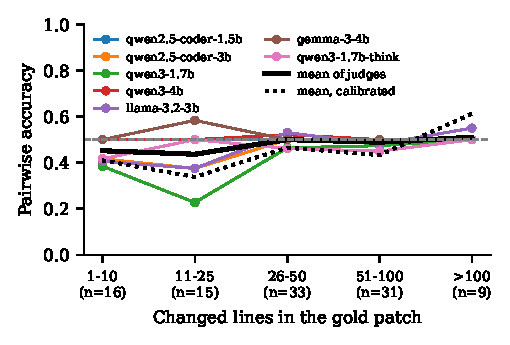
\includegraphics[width=\columnwidth]{../results/figures/scaling.pdf}
\caption{Accuracy by gold-patch size (changed lines); bin sizes in parentheses.
The dotted line is the judges' mean after position calibration.}
\label{fig:scaling}
\end{figure}

\input{generated/tab_scaling.tex}

\subsection{Defect-class error profile (O4)}
\label{sec:res-classes}

\Cref{tab:classes} breaks accuracy down by class.  \ClassText{}

\input{generated/tab_classes.tex}

\subsection{Mitigation: repository context, and thinking (O6)}
\label{sec:res-context}

\Cref{tab:context} compares context-augmented prompts with the diff-only
prompt on the same pairs.  \ContextText{}

\input{generated/tab_context.tex}

\subsection{Baselines and point-wise judging}
\label{sec:res-baselines}

\Cref{tab:baselines} lists the non-LLM baselines.  \BaselineText{}

\input{generated/tab_baselines.tex}



\subsection{Threats to validity}
\label{sec:threats}

\textbf{Construct validity.}  Our defects are injected by operators, not
collected from real rejected pull requests, so their distribution follows the
operators and the constructs that happen to occur near the patched code.  Some
operators leave local cues that a pattern matcher can exploit (for example
\texttt{except Exception: pass}); the static-analysis baseline measures how far
such cues go.  The plausibility and the defectiveness of the variants were not
validated by human annotators.

\textbf{Internal validity.}  The admission filter runs the PR's relevant test
files rather than the whole suite; a variant could in principle break a test
elsewhere in the repository, which would make the task easier for an execution
oracle but does not change what the judge sees.  Docker images were pulled
through a public registry mirror and are the images published with the tasks.

\textbf{Judges and prompting.}  All judges are small (1.5--4B), quantised
(4--8 bit) open models.  In the main condition they must answer without first
writing an explanation; the base paper lets judges reason before the verdict,
so our direct-verdict numbers are a lower bound for these models, and the
thinking condition measures how much reasoning recovers.

\textbf{Statistical conclusion validity.}  The benchmark is small, rare classes
have few pairs, and pairs built from the same pull request are correlated; we
therefore resample tasks rather than pairs in the bootstrap and report
intervals rather than significance stars.  We do not correct for multiple
comparisons; per-class and per-condition differences should be read as
exploratory.

\textbf{Selection.}  Pairs whose diff-only prompt exceeds the judges' token
budget, and tasks with solution leakage, are excluded from judging, which caps
the diff sizes the scaling analysis can observe.


\section{Conclusion}
\label{sec:conclusion}

We introduced \RJB{}, a benchmark of \NPairs{} execution-verified
(gold patch, defective variant) pairs built from real pull requests created
after 1~January~2025, in which every defective variant keeps all of the PR's
gold-passing tests green.  Constructing it showed that the PR's tests catch only
\TestCatchRate{} of review-relevant injected defects, so a test-based oracle
cannot separate the two patches by construction.

\ConclusionJudges{}

Three lessons follow.  First, the reliability problems that \CJB{} reports for
single-file code---sensitivity to presentation order---do not disappear at
repository level; for small open judges they dominate the verdict.  Second,
judges must be audited for \emph{length} preferences: on our pairs the
defective patch is usually the longer one, and judges systematically prefer it,
while a trivial shorter-patch rule scores \LengthHeurAcc{}.  This is also a
lesson for benchmark builders, ourselves included: the next version of
\RJB{} should length-match each variant to its gold patch.  Third, cheap,
targeted static analysis (\StaticRelAcc{}) is a strong baseline that any
execution-free judge for code review should be required to beat.

\textbf{Future work.}  Length-matched variants and naturally occurring
defective PRs; Django- and SQLAlchemy-heavy repositories to populate the N+1
and migration classes; per-instance witness tests; the planned two-annotator
validation; and frontier (closed and large open) judges, for which our harness
only needs an API backend.


\bibliographystyle{IEEEtran}
\bibliography{references}

\end{document}
